\documentclass{beamer}
\usepackage{float}
\usepackage{multicol}
\usepackage{bm}
\usepackage{amsmath,amsthm,amsfonts,amssymb,amscd, fancyhdr, color, comment, graphicx, environ}

\addtobeamertemplate{navigation symbols}{}{%
    \usebeamerfont{footline}%
    \usebeamercolor[fg]{footline}%
    \hspace{1em}%
    \insertframenumber/\inserttotalframenumber
}

%Information to be included in the title page:
\title{Diffusion-based Vocoding for Real-Time Text-To-Speech}
\author{Lukas Gardberg}
\institute{LTH}
\date{\today}

\begin{document}

\frame{\titlepage}

\begin{frame}
\frametitle{Presentation Layout}
\begin{itemize}
    \item Problem Introduction
    \item Past Work
    \item Problem Statement
    \item Diffusion Models
    \item Improvements
    \item Method \& Results
    \item Discussion \& Future Work
\end{itemize}
\end{frame}

% ---------- %

\begin{frame}
\frametitle{Typical TTS Pipeline}

\vspace{1cm}

\begin{center}
{\large
    Text \quad $\longrightarrow$ \quad Speech
}
\end{center}

\vspace{1cm}

\pause

\begin{figure}[H]
    \centering
    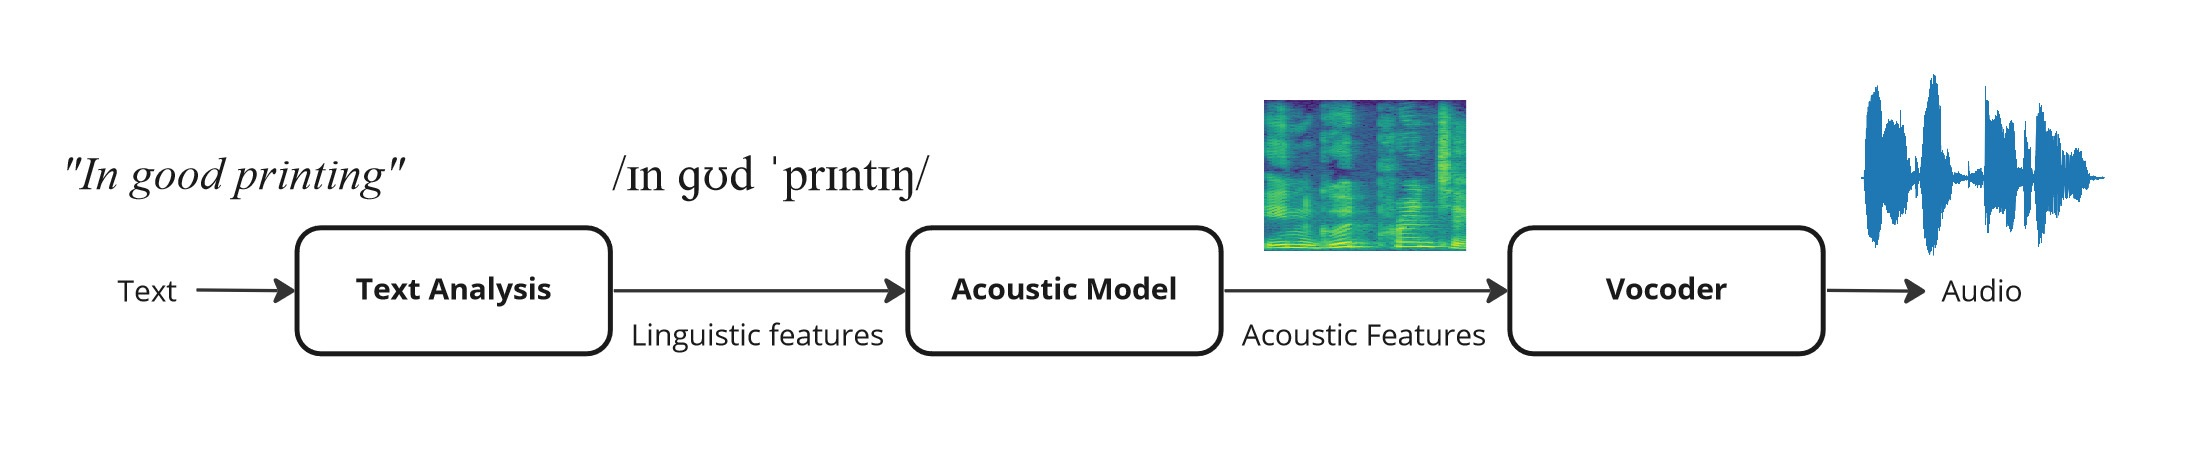
\includegraphics[width=1\textwidth]{images/TTS.jpg}
\end{figure}

\vspace{1cm}

\begin{multicols}{3}
    \begin{center}

    Text Analysis

    \vfill\null
    \columnbreak

    Acoustic Model

    \vfill\null
    \columnbreak

    Vocoder

    \end{center}
\end{multicols}

\end{frame}

% ---------- %

\begin{frame}
    \frametitle{The Phase Reconstruction Problem}

    \begin{itemize}
        \item Goal: Reconstruct signal $\bm{x}$ from its mel spectrogram $\bm{S}_{\text{mel}}$
    \end{itemize}
    
    \pause

    \begin{figure}[H]
        \centering
        \includegraphics[width=1\textwidth]{images/Phase_reconstruction.png}
    \end{figure}
    
\end{frame}

% ---------- %

\begin{frame}
    \frametitle{The Phase Reconstruction Problem}

    How has this been done before?

    \vspace{1cm}

    \begin{itemize}
        \pause
        \item Griffin-Lim Reconstruction
        \pause
        \item Autoregressive Neural Networks (WaveNet)
        \pause
        \item GANs (HiFi-GAN)
        \pause
        \item Diffusion (DiffWave)
        \pause
        \item ...and more
    \end{itemize}
    
    
\end{frame}

% ---------- %

\begin{frame}{Problem Statement}
    
    \begin{itemize}
        \setlength\itemsep{1em}
        \item How does inference speed and generated audio quality compare to a GAN-based vocoder?
        \pause
        \item How do the following aspects affect inference speed and audio quality?
        \pause
        \begin{itemize}
            \item Variance schedule
            \item Time-step importance sampling 
            \item Noise prior
        \end{itemize}
        \pause
        \item How does a vocoder trained on audio from one speaker generalize to another?
        \pause
        \item Can such a model generate audio faster than real-time?
    \end{itemize}
    
\end{frame}

% ---------- %

\begin{frame}{Diffusion}
\large
    \begin{itemize}
        \setlength\itemsep{1.5em} 
        \item How can it be used for vocoding?
    \end{itemize}

\end{frame}    

% ---------- %

\begin{frame}{Diffusion}

    \begin{itemize}
        \setlength\itemsep{1.5em}
        \item Transform data from $q_{\text{data}}$ into a simple distribution $p_{\text{latent}}$ ("forward process")
        \pause
        \item Learn to transform data from a simple distribution $p_{\text{latent}}$ (e.g. noise) into the complex target distribution $q_{\text{data}}$ ("backward process")
        \pause
        \item Teach a model to perform the inverse transformation in several steps
    \end{itemize}

\end{frame}

% ---------- %

% \begin{frame}{Forward Process}

% $T$: Number of diffusion steps \\
% \pause
% $\bm{x}_0$: Ground truth sample \\
% \pause
% $\bm{x}_t$: Sample after $t$ diffusion steps \\
% \pause
% $\bm{x}_T$: Final sample, hopefully close to $p_{\text{latent}}$ \\

% \vspace{0.4cm}

% Generating a noisy sample:
% \pause

% \begin{align*}
% \bm{x}_t \sim & \, q(\bm{x}_t \mid \bm{x}_{t-1}) = \, \mathcal{N}(\bm{x}_t \, ; \, \sqrt{1 - \beta_t} \bm{x}_{t-1}, \beta_t \bm{I}) \\
% \bm{x}_t = & \, \sqrt{1 - \beta_t} \bm{x}_{t-1} + \beta_t \bm{\varepsilon}, \quad \bm{\varepsilon} \sim \mathcal{N}(\bm{0}, \bm{I}) \\
% \end{align*}

% \vspace{0.4cm}

% \pause

% Variance schedule $\beta_t \in [0, 1]$: At which "rate" we tend towards a unit Gaussian

% \end{frame}

% ---------- %

\begin{frame}{Forward Process}

    \begin{figure}[H]
        \centering
        \includegraphics[width=0.79\textwidth]{images/density2.png}
    \end{figure}

\end{frame}

% ---------- %

\begin{frame}{Forward Process}

    \begin{itemize}
        \setlength\itemsep{1.5em}
        \item Choose a number of diffusion steps $T$
        \item Decide how "big" steps we take via a variance schedule $\beta_t$
        \item Each sample is drawn as $q(\bm{x}_t \mid \bm{x}_{t-1}) = \, \mathcal{N}(\bm{x}_t \, ; \, \sqrt{1 - \beta_t} \bm{x}_{t-1}, \beta_t \bm{I})$ 
    \end{itemize}
    
\end{frame}

% ---------- %
% 
% \begin{frame}{Forward Process}
%     Quick way to get a noisy sample $\bm{x}_t$:

%     \vspace{0.6cm}

%     \begin{align*}
%         \bar{\alpha}_t = & \, \prod_{i=1}^t (1 - \beta_i) \\
%         \bm{x}_t \sim & \ q(\bm{x}_t \mid \bm{x}_{0}) = \mathcal{N}(\bm{x}_t \, ; \, \sqrt{\bar{\alpha}_t} \bm{x}_0, \sqrt{1-\bar{\alpha}_t} \bm{I}), \\
%         \bm{x}_t = & \, \sqrt{\bar{\alpha}_t} \bm{x}_0 + \sqrt{1-\bar{\alpha}_t} \bm{\varepsilon}, \quad \bm{\varepsilon} \sim \mathcal{N}(\bm{0}, \bm{I}) \\
%     \end{align*}
    
% \end{frame}

% ---------- %

\begin{frame}{Backward Process}

\begin{itemize}
    \setlength\itemsep{1.5em}
    \item We want to be able to generate samples by reversing the process
    \pause
    \item Model each transition as $p_{\theta}(\bm{x}_{t-1} \mid \bm{x_t})$, model is to predict the noise added in each step via $\bm{\varepsilon}_{\theta}$ % = \mathcal{N}(\bm{x}_{t-1} \, ; \, \bm{\mu}_{\theta}(\bm{x}_t, t), \bm{\Sigma}_{\theta}(\bm{x}_t, t))$
    \pause
    \item We condition on more noisy sample $\bm{x}_t$, diffusion step $t$, and the mel-spectrogram $\bm{S}_{\text{mel}}$ in each step
    \pause
    \item Training: sample $t$ uniformly over $[1, T]$
\end{itemize}
    
\end{frame}

% ---------- %

\begin{frame}{Backward Process}

    \begin{figure}[H]
        \centering
        \includegraphics[width=0.79\textwidth]{images/density.png}
    \end{figure}

\end{frame}

% ---------- %

% \begin{frame}{Backward Process}

% In practice:

% \begin{itemize}
%     \setlength\itemsep{1.5em}
%     \item Discard $\bm{\Sigma}_{\theta}$ as learnable (simplification)
    % \pause
%     \item Let the inputs to the model be $\bm{x}_t$, $t$, and $\bm{S}_{\text{mel}}$ in each step
%     \pause
%     \item Let the model predict the added noise instead of the mean: $\bm{\varepsilon}_{\theta}(\bm{x}_t, t, \bm{S}_{\text{mel}})$
%     \pause
%     \item Each backwards step is a denoising step
% \end{itemize}

% \end{frame}

% ---------- %

\begin{frame}{Backward Process}

    \begin{figure}[H]
        \centering
        \includegraphics[width=0.79\textwidth]{images/viper.png}
    \end{figure}

\end{frame}

% ---------- %

% \begin{frame}{Backward Process}

%     Loss Function:

%     $$
%     L_{\text{simple}} = \mathbb{E}_{t, \bm{x}_0, \bm{\varepsilon}} \|\bm{\varepsilon} - \bm{\varepsilon}_\theta\|^2_1 
%     $$

%     \begin{itemize}
%         \item Learn to take a single backward step based on samples from the forward process
%         \pause
%         \item $\bm{\varepsilon}$ is the noise added in the forward process, and $\bm{\varepsilon}_\theta$ is the noise subtracted in the backward process
%         \pause
%         \item Training: sample $t$ uniformly over $[1, T]$
%     \end{itemize}
 

% \end{frame}

% ---------- %

\begin{frame}{Main Considerations}

    \begin{itemize}
        \setlength\itemsep{1.5em}
        \item Choice of variance schedule $\beta_t$
        \pause
        \item Choice of noise prior $p_{\text{latent}}$
        \pause
        \item Uniform vs importance sampling of $t$
    \end{itemize}

\end{frame}

% ---------- %

\begin{frame}{Variance Schedule}

    \begin{itemize}
        \item We do not want to reach white noise too early
        \item Smooth transition from data to noise
    \end{itemize}

    \begin{figure}[H]
        \centering
        \includegraphics[width=1\textwidth]{images/schedules.png}
    \end{figure} 

\end{frame}

% ---------- %

% \begin{frame}{Variance Schedule}
%    Inverse Quadratic Schedule: $ \bar{\alpha}_t = 1 - \left(\frac{t}{T}\right)^2$ \\ 
%    \vspace{0.5cm}
%    Linear noise factor in $\bm{x}_t = \sqrt{\bar{\alpha}_t} \bm{x}_0 + \sqrt{1-\bar{\alpha}_t} \bm{\varepsilon}$ \\
%    \vspace{0.5cm}
%    Similar to original linear, but reaches $\bar{\alpha}_t = 0$
% \end{frame}

% ---------- %

\begin{frame}{Importance Sampling}

    \vspace{0.5cm}

    Gradient is noisy when training! Most likely from a skewed loss:

    \begin{figure}[H]
        \centering
        \includegraphics[width=0.7\textwidth]{images/time_step_loss.png}
    \end{figure}

    Hypothesis: some steps are harder to learn than others \\
    \vspace{0.5cm}
    Idea: sample $t$ weighted by the loss 
    
\end{frame}

% ---------- %

\begin{frame}{Choice of Prior}
    \vspace{0.2cm}

    Instead of starting from unit white noise, can we choose a better prior?
    
    \pause

    \begin{itemize}
        \item Use information from $\bm{S}_{\text{mel}}$ to choose a prior
        \pause
        \item Get variance of starting noise from frame-level energy of $\bm{S}_{\text{mel}}$
    \end{itemize}
    
    \pause

    \begin{figure}[H]
        \centering
        \includegraphics[width=0.9\textwidth]{images/priornoise.png}
    \end{figure}

\end{frame}

% ---------- %

\begin{frame}{Choice of Prior}

    \begin{figure}[H]
        \centering
        \includegraphics[width=0.7\textwidth]{images/priorgrad_image1.png}
    \end{figure}
    
\end{frame}

% ---------- METRICS ---------- %

\begin{frame}{Metrics}

    \begin{itemize}
        \setlength\itemsep{1.5em}
        \item Approximate Mean Opinion Score (AMOS)
        \begin{itemize}
            \item Scale 1-5, finetuned audio model 
        \end{itemize}
        \item Log-mel Spectrogram Mean Absolute Error (LS-MAE)
        \item Peak Signal-to-Noise Ratio (PSNR)
        \item Multi-resolution STFT Error (MRSE)
    \end{itemize}

\end{frame}

% ---------- DATA ---------- %

\begin{frame}{Data}
\large
    \begin{itemize}
        \setlength\itemsep{1.5em}
        \item LJ Speech
        \begin{itemize}
            \setlength\itemsep{0.5em}
            \item Training set
            \item 24 hours of speech from audiobooks 
            \item 13 100 audio files, 95 in test set
            \item Sample rate: 22 050 Hz
        \end{itemize}
        \item LibriTTS
        \begin{itemize}
            \setlength\itemsep{0.5em}
            \item Test set of other speaker
            \item 515 audio files
        \end{itemize}
    \end{itemize}
    
\end{frame}

% ---------- MODEL ---------- %

\begin{frame}{Model}

\begin{itemize}
    \setlength\itemsep{1.5em}
    \item DiffWave, based on dilated convolutions
    \item 2.6M parameters, $T=50$
    \item Short inference schedule with $T=6$
\end{itemize}
    
\end{frame}


% ---------- METHOD & RESULTS ---------- %

\begin{frame}{Method \& Results}

    Experiments

    \vspace{0.5cm}

    \begin{itemize}
        \setlength\itemsep{1.5em}
        \item Variance Schedules
        \item Time-step Sampling
        \item Noise Prior
        \item Model Size
        \item Inference Speed
        \item Longer Training
    \end{itemize}
    
\end{frame}

% ---------- %

\begin{frame}{Method \& Results: Variance Schedule}

Objective Metrics:

    \begin{figure}[H]
        \centering
        \includegraphics[width=1\textwidth]{images/table_scheds_o.png}
    \end{figure}

\end{frame}

% ---------- %

\begin{frame}{Method \& Results: Variance Schedule}

Subjective Metrics:

    \begin{figure}[H]
        \centering
        \includegraphics[width=0.9\textwidth]{images/table_scheds.png}
    \end{figure}
    
\end{frame}

% ---------- %

\begin{frame}{Method \& Results: Variance Schedule}

    \begin{itemize}
        \setlength\itemsep{1.5em}
        \item Original Linear and Inverse Quadratic best
        \pause
        \item Scaled surprisingly bad
        \pause
        \item Griffin Lim best objective metrics, worst AMOS
    \end{itemize}
\end{frame}

% ---------- %

\begin{frame}{Method \& Results: Time-step Sampling}

    \begin{figure}
        \centering
        \includegraphics[width=1\textwidth]{images/weighted_loss_variance.png}
    \end{figure}

\end{frame}

% ---------- %

\begin{frame}{Method \& Results: Time-step Sampling}

Objective Metrics:

    \begin{figure}[H]
        \centering
        \includegraphics[width=1\textwidth]{images/table_imps_o.png}
    \end{figure} 

\end{frame}

% ---------- %

\begin{frame}{Method \& Results: Time-step Sampling}

Subjective Metrics:

    \begin{figure}[H]
        \centering
        \includegraphics[width=1\textwidth]{images/table_imps_a.png}
    \end{figure}

\end{frame}

% ---------- %

\begin{frame}{Method \& Results: Time-step Sampling}

    \begin{itemize}
        \setlength\itemsep{1.5em}
        \item Loss variance reduced
        \pause
        \item Both objective \& subjective scores similar
        \pause
        \item Not significantly more robust to shorter schedule
    \end{itemize}

\end{frame}

% ---------- %

\begin{frame}{Method \& Results: Noise Prior}

Objective Metrics:

    \begin{figure}[H]
        \centering
        \includegraphics[width=1\textwidth]{images/table_prior_o.png}
    \end{figure}

\end{frame}

% ---------- %

\begin{frame}{Method \& Results: Noise Prior}

Subjective Metrics:

    \begin{figure}[H]
        \centering
        \includegraphics[width=1\textwidth]{images/table_prior_a.png}
    \end{figure}

\end{frame}

% ---------- %

\begin{frame}{Method \& Results: Noise Prior}

    \begin{itemize}
        \setlength\itemsep{1.5em}
        \item Both objective and subjective scores improved
        \pause
        \item Slightly worse performance for short schedule
        \pause
        \item Higher MRSE might indicate overfitting
    \end{itemize}

\end{frame}

% ---------- %

\begin{frame}{Method \& Results: Model Size}

    How does model size affect performance?

    \vspace{0.5cm}

    Objective Metrics:

    \begin{figure}
        \centering
        \includegraphics[width=1\textwidth]{images/table_size_o.png}
    \end{figure}

\end{frame}

% ---------- %

\begin{frame}{Method \& Results: Model Size}

    Subjective Metrics:

    \begin{figure}
        \centering
        \includegraphics[width=1\textwidth]{images/table_size_a.png}
    \end{figure}

\end{frame}

% ---------- %

\begin{frame}{Method \& Results: Model Size}

    \begin{itemize}
        \setlength\itemsep{1.5em}
        \item 70\% model size, only 75\% of inference time
        \pause
        \item Minimal difference in audio quality
        \pause
        \item IQ + IS did not result in a better smaller model
    \end{itemize}

\end{frame}

% ---------- %

\begin{frame}{Method \& Results: Inference Speed}

    How do the models compare in terms of inference speed?

    \vspace{0.5cm}

    \begin{figure}
        \centering
        \includegraphics[width=0.9\textwidth]{images/rtfs.png}
    \end{figure}

\end{frame}

% ---------- %

\begin{frame}{Method \& Results: Inference Speed}

    \begin{itemize}
        \setlength\itemsep{1.5em}
        \item Slowest: PriorGrad, 60x slower than real-time on CPU, 0.55x on GPU
        \pause
        \item Fastest: Small Diffwave (fast), 4x slower than real-time on CPU, 0.05x on GPU
        \pause
        \item Fast sampling: 12\% of steps, 9x speedup
        \pause
        \item Still 15 times slower than HiFi-GAN
    \end{itemize}

\end{frame}

% ---------- %

\begin{frame}{Method \& Results: Longer Training}

    How does longer training affect performance?

    \vspace{0.5cm}

    Objective Metrics:

    \begin{figure}
        \centering
        \includegraphics[width=1\textwidth]{images/table_long_o.png}
    \end{figure}

\end{frame}

% ---------- %

\begin{frame}{Method \& Results: Longer Training}

    Subjective Metrics:

    \begin{figure}
        \centering
        \includegraphics[width=1\textwidth]{images/table_long_a.png}
    \end{figure}

\end{frame}

% ---------- %

\begin{frame}{Method \& Results: Longer Training}

    \begin{itemize}
        \setlength\itemsep{1.5em}
        \item 5x longer training, only slightly better scores
        \pause
        \item Similar quality to HiFi-GAN
        \pause
        \item IQ + IS resulted in similar scores to base

    \end{itemize}

\end{frame}

% ---------- %

\begin{frame}{Method \& Results: Recap}

    \begin{itemize}
        \setlength\itemsep{1em}
        \item Variance Schedule: Original Linear \& IQ similar, image generation schedules worse
        \pause
        \item Time-step Sampling: Lower variance, no change in performance
        \pause
        \item Noise Prior: Improved performance
        \pause
        \item Smaller Model: slightly faster, quality approximately the same
        \pause
        \item Inference Speed: Fastest 0.05x RTF on GPU, 4x on CPU
        \pause
        \item Longer Training: 5x longer training, similar scores
    \end{itemize}

\end{frame}

% ---------- %

\begin{frame}{Discussion}

    Main takeaways:

    \begin{itemize}
        \setlength\itemsep{1em}
        \item Possible to perform vocoding using diffusion on GPU, slow on CPU, further speedup possible
        \pause 
        \item Choice of schedule important, should not reach noise too early
        \pause
        \item Importance sampling: not more robust, but better variance
        \pause
        \item Able to generalize to another speaker, AMOS hard to interpret
        \pause
        \item Objective Metrics not always reliable
        \pause
        \item Similar quality to HiFi-GAN, but slower

    
    \end{itemize}
    
\end{frame}

% ---------- %

\begin{frame}{Future Work}

    \begin{itemize}
        \setlength\itemsep{1em}
        \item IQ + IS + PriorGrad
        \pause
        \item Better theoretical understanding of the schedule is needed
        \pause
        \item Learnable $\bm{\Sigma}_{\theta}$, condition on $\bar{\alpha}_t$
        \pause
        \item Smaller model, shorter schedule
        \pause
        \item Better metrics
        \pause
        \item Higher sample rate, Distillation, Super-resolution 
    \end{itemize}
    
\end{frame}

% ---------- %

\begin{frame}

    \Large

    \centering

    \vspace{1.5cm}

    Thank you!
    
\end{frame}

\end{document}